\subsection{Overview}

Our methodology consists of three components: (1) the Decisive Shock Score (DSS), which quantifies the role of decisive battles or campaigns in determining war outcomes; (2) the Strategic Exhaustion Score (SES), which measures the cumulative attritional dynamics of prolonged conflict; and (3) a dynamical simulation model that generates synthetic war trajectories under varying parameter regimes. Together, these components enable us to test whether the ``decisive battle'' or ``attrition'' hypothesis better explains historical patterns of war termination.

\subsection{Dimensionless Normalized State Variables}

All state variables in the simulation model are \textbf{dimensionless normalized indices}, not physical quantities. A value of 100 represents the preset side's initial or maximum normalized capacity, not a measured troop count, GDP value, or population count. The update-equation coefficients are therefore \emph{scale coefficients} in a bounded discrete-time map, not physical constants with units. This normalization means that equation terms are internally consistent within the $[0, 100]$ state space but do not carry physical units across equations. We make this explicit to avoid dimensional-analysis objections: the model is a bounded iterative map, not a system of differential equations with physical dimensions.

\subsection{Decisive Shock Score (DSS)}

The Decisive Shock Score is a composite metric that captures the degree to which a war's outcome is attributable to a decisive battle, campaign, or shock event. DSS is computed from nine weighted components, each capturing a different aspect of decisive impact:

\begin{equation}
\text{DSS} = \sum_{i=1}^{9} w_i \cdot s_i
\label{eq:dss}
\end{equation}

\noindent where $w_i$ are weights summing to 1.0, and $s_i$ are normalized component scores in $[0, 1]$. The nine components are:

DSS and SES are composite indices from weighted component scores. Weights are heuristic priors, not empirically fitted. DSS weights are in Table~\ref{tab:component_availability}; SES weights are in the source code. Components within each index may be correlated. Scores should be interpreted ordinally, not as interval-scale truth.

\begin{enumerate}
    \item \textbf{Concentration Ratio} ($w_1 = 0.20$): Proportion of total war casualties in the single largest battle.
    \item \textbf{Temporal Clustering} ($w_2 = 0.15$): Degree to which casualty-producing events are clustered in time, computed as the inverse of the coefficient of variation of inter-battle intervals.
    \item \textbf{Force Ratio at Peak} ($w_3 = 0.12$): Ratio of forces engaged in the largest battle to total forces deployed.
    \item \textbf{Outcome Proximity} ($w_4 = 0.18$): Temporal proximity between the largest battle and war termination.
    \item \textbf{Morale Cascade Index} ($w_5 = 0.10$): Whether the largest battle precipitated rapid collapse in the losing side's ability to fight.
    \item \textbf{Territorial Swing} ($w_6 = 0.10$): Magnitude of territorial change following the largest battle relative to total territorial change.
    \item \textbf{Force Destruction Ratio} ($w_7 = 0.08$): Fraction of the losing side's total military capability destroyed in a single engagement.
    \item \textbf{Surprise Index} ($w_8 = 0.04$): Ratio of forces at the point of attack to the defender's expectation.
    \item \textbf{Alliance Cascade} ($w_9 = 0.03$): Whether the decisive battle triggered defections among alliance partners.
\end{enumerate}

DSS values range from 0 (no decisive battle dynamics) to 100 (maximally decisive single-event dynamics). Components $w_4$ (Outcome Proximity), $w_5$ (Morale Cascade), and $w_6$ (Territorial Swing) require post-hoc knowledge of war outcomes. These components are retained for explanatory power but should not be interpreted as exogenous predictors.

Table~\ref{tab:component_availability} classifies each DSS component by when its information becomes available to a strategic observer.

\begin{table}[H]
\centering
\caption{DSS component classification by information availability. ``Outcome-dependent'' components require knowledge of the war's outcome and contribute to the observed-structural DSS gap.}
\label{tab:component_availability}
\small
\setlength{\tabcolsep}{2pt}
\renewcommand{\arraystretch}{1.05}
\begin{tabularx}{\textwidth}{l c l X}
\toprule
\textbf{Component} & \textbf{Weight} & \textbf{Availability} & \textbf{Rationale} \\
\midrule
Concentration Ratio & 0.20 & Outcome-dependent & Share of total casualties in the single largest battle \\
Temporal Clustering & 0.15 & Outcome-dependent & Full timeline of battle events needed \\
Force Ratio at Peak & 0.12 & Early-war & Partially estimable early; precise only after the battle \\
Outcome Proximity & 0.18 & Post-hoc & Distance between largest battle and war end \\
Morale Cascade Index & 0.10 & Post-hoc & Collapse rate after largest battle \\
Territorial Swing & 0.10 & Post-hoc & Territorial change after largest battle \\
Force Destruction Ratio & 0.08 & Outcome-dependent & Fraction of capability destroyed in one engagement \\
Surprise Index & 0.04 & Early-war & Partially estimable from force positioning \\
Alliance Cascade & 0.03 & Post-hoc & Alliance defections only observable after diplomatic events \\
\bottomrule
\end{tabularx}
\end{table}

\subsection{Strategic Exhaustion Score (SES)}

The Strategic Exhaustion Score measures the degree to which a war's outcome is associated with cumulative attrition and exhaustion. SES is computed from ten weighted components:

\begin{equation}
\text{SES} = \sum_{j=1}^{10} v_j \cdot e_j
\label{eq:ses}
\end{equation}

\noindent where $v_j$ are weights summing to 1.0, and $e_j$ are normalized component scores in $[0, 1]$. As with DSS, components within SES may be correlated and weights are heuristic priors. The ten components are:

\begin{enumerate}
    \item \textbf{Cumulative Mortality} ($v_1 = 0.18$): Total battle deaths as a fraction of the losing side's pre-war population, capturing the human cost of prolonged conflict.
    \item \textbf{Duration Percentile} ($v_2 = 0.15$): War duration relative to the distribution of all wars in the dataset, normalized to $[0, 1]$.
    \item \textbf{Economic Drain Index} ($v_3 = 0.14$): Ratio of peak military expenditure to pre-war GDP, capturing the economic burden of sustained warfare.
    \item \textbf{Manpower Depletion} ($v_4 = 0.12$): Rate of decline in available military manpower over the course of the war.
    \item \textbf{Territorial Attrition} ($v_5 = 0.10$): Gradual loss of territory over time, measured as the rate of decline in controlled territory.
    \item \textbf{Force Ratio Trajectory} ($v_6 = 0.09$): Trend in the ratio of opposing forces over time, capturing whether the balance of power shifts gradually.
    \item \textbf{Logistics Strain} ($v_7 = 0.08$): Measure of supply difficulty, estimated from the ratio of forces to supply capacity.
    \item \textbf{Morale Decay Rate} ($v_8 = 0.06$): Rate of decline in fighting effectiveness, estimated from desertion rates or surrender frequency.
    \item \textbf{Political Will Erosion} ($v_9 = 0.05$): Measure of declining domestic support for the war, estimated from regime stability indicators.
    \item \textbf{Cumulative Cost Ratio} ($v_{10} = 0.03$): Ratio of cumulative costs borne by the two sides, capturing asymmetric exhaustion.
\end{enumerate}

SES values range from 0 (no exhaustion dynamics) to 100 (maximally attritional dynamics). For conflicts where battle-level data is unavailable, we estimate missing components from aggregate war-year data using regression imputation models trained on wars with complete data.

\subsection{Hybrid Classification Rule}

To classify wars into termination types, we combine DSS and SES using a hybrid rule that accounts for the possibility that both mechanisms operate simultaneously:

\begin{equation}
\text{Termination Type} = \begin{cases}
    \text{Data Insufficient} & \text{if both DSS and SES are unavailable} \\
    \text{Uncertain} & \text{if } \max(\text{DSS}, \text{SES}) < 45 \\
    \text{Mixed} & \text{if both DSS} \geq 65 \text{ and SES} \geq 65 \\
    \text{Decisive Shock} & \text{if } \text{DSS} - \text{SES} \geq 20 \\
    \text{Strategic Exhaustion} & \text{if } \text{SES} - \text{DSS} \geq 20 \\
    \text{Mixed/Uncertain} & \text{otherwise}
\end{cases}
\label{eq:hybrid}
\end{equation}

This classification is deliberately conservative: wars with strong dynamics on both dimensions are classified as ``Mixed'' rather than forced into a single category. Our analysis examines the distribution of these classifications and the features that predict each type.

\subsection{War Dynamics Simulation Model}\label{sec:simulation}

We construct a dynamical simulation model that generates synthetic war trajectories under varying parameter regimes. The model operates on a discrete time grid $t \in \{0, 1, 2, \ldots, T\}$, where each time step represents one month of simulated time. The simulator is implemented as the \texttt{WarSimulator} class in the project source code. Like all simulation models, it is a simplified representation of reality; its value lies in demonstrating that the proposed mechanisms can generate internally consistent trajectories, not in producing definitive historical predictions.

\subsubsection{State Variables}

Each simulation maintains five state variables for each side (A and B), all clamped to $[0, 100]$:

\begin{tabular}{@{}lll@{}}
\textbf{Variable} & \textbf{Side A} & \textbf{Side B} \\
\midrule
Military strength & $\text{Mil}_A(t)$ & $\text{Mil}_B(t)$ \\
Economic capacity & $\text{Econ}_A(t)$ & $\text{Econ}_B(t)$ \\
Political will & $\text{Pol}_A(t)$ & $\text{Pol}_B(t)$ \\
Population support & $\text{Pop}_A(t)$ & $\text{Pop}_B(t)$ \\
Industrial capacity & $\text{Ind}_A(t)$ & $\text{Ind}_B(t)$ \\
\end{tabular}

\subsubsection{Attrition Update Equations}

At each time step, attrition is applied symmetrically to both sides. The attrition rate parameter $\rho \in [0, 100]$ is normalized to $\bar{\rho} = \rho / 100$, and a cumulative fatigue factor $f(t)=\min(f_{\max}, 1+t/60)$ with $f_{\max}=2.5$ captures increasing difficulty of sustained operations. Economic resilience $\tau$ modulates damage susceptibility via a resistance factor $r = 1 - \tau/200 \in [0.5, 0.75]$.

\begin{align}
\text{Mil}(t+1) &= \text{Mil}(t) - \text{Mil}(t) \cdot \bar{\rho} \cdot 0.04 \cdot r \cdot f(t) + \min(1.5, \text{Ind}(t) \cdot 0.004) \label{eq:sim_mil} \\
\text{Econ}(t+1) &= \text{Econ}(t) - \text{Econ}(t) \cdot \bar{\rho} \cdot 0.025 \cdot f(t) \notag \\
&\quad - \text{Econ}(t) \cdot \bar{\rho} \cdot 0.01 \cdot r + \text{Ind}(t) \cdot 0.006 \label{eq:sim_econ} \\
\text{Pol}(t+1) &= \text{Pol}(t) - \Delta\text{Mil} \cdot 0.2 - \bar{\rho} \cdot 0.4 \cdot f(t) \cdot (1 - \pi/200) + v(t) \label{eq:sim_pol} \\
\text{Pop}(t+1) &= \text{Pop}(t) - \max(0, 50 - \text{Econ}(t)) \cdot \bar{\rho} \cdot 0.03 \cdot f(t) \notag \\
&\quad - 0.03 \cdot \Delta\text{Mil} \label{eq:sim_pop} \\
\text{Ind}(t+1) &= \text{Ind}(t) - \text{Ind}(t) \cdot \bar{\rho} \cdot 0.015 \cdot r \cdot f(t) + \text{Econ}(t) \cdot 0.004 \label{eq:sim_ind}
\end{align}

\noindent where $\Delta\text{Mil}$ is the battle loss computed in Equation~\ref{eq:sim_mil}, $\pi$ is the political resilience parameter, and the political advantage term is smooth rather than binary:
\[
v_s(t)=\gamma_w \max\left(0,\frac{\text{Mil}_s(t)-\text{Mil}_{\neg s}(t)}{\text{Mil}_s(t)+\text{Mil}_{\neg s}(t)+\epsilon}\right),
\]
where $\gamma_w=0.15$ for limited wars and $\gamma_w=0.8$ otherwise, and $\epsilon=1$ prevents division by zero.

\subsubsection{Shock Events (Decisive Shock Mechanism)}

Decisive shocks are applied periodically at an interval determined by the war type: every 3 months for limited wars, 6 for total wars, and 7 for coalition wars. The shock magnitude is $\sigma = \text{shock\_strength} / 100 \in [0, 1]$.

Each side applies a shock proportional to its side-specific shock strength $\sigma_s$:
\begin{align}
\text{Mil}_{\neg s}(t) &\leftarrow \text{Mil}_{\neg s}(t) - \sigma_s \cdot 8.0 \\
\text{Ind}_{\neg s}(t) &\leftarrow \text{Ind}_{\neg s}(t) - \sigma_s \cdot 8.0 \cdot \eta_{\text{ind},s} \\
\text{Pol}_{\neg s}(t) &\leftarrow \text{Pol}_{\neg s}(t) - \sigma_s \cdot 8.0 \cdot \eta_{\text{pol},s}
\end{align}

\noindent where $\neg s$ denotes the opposing side. For Side~A, $\eta_{\text{ind}}=0.30$ and $\eta_{\text{pol}}=0.25$; for Side~B, $\eta_{\text{ind}}=0.25$ and $\eta_{\text{pol}}=0.20$ in the current calibrated implementation.

\noindent with analogous reductions to military, industrial, and political state variables. After both attrition and shock updates, independent Gaussian noise $\mathcal{N}(0, 0.5)$ is added to all state variables to model exogenous perturbations. All states are clamped to $[0, 100]$.

\subsubsection{Observed versus Structural DSS Proxy}

A fundamental methodological distinction underlies this paper: the difference between \emph{observed} DSS and \emph{structural DSS proxy}. These answer different scientific questions and must not be conflated.

The \textbf{observed DSS} (Equation~\ref{eq:dss}) answers: ``Given what happened, how much did decisive events contribute to termination?'' This metric incorporates post-hoc information, outcome proximity, morale cascade, and territorial swing, and therefore includes information unavailable before the outcome. It is useful for \emph{explaining} historical outcomes but cannot be used for \emph{forecasting}.

The \textbf{structural DSS proxy} answers: ``Before the outcome was known, how much structural evidence existed for decisive mechanisms?'' This metric uses only exogenous, pre-outcome features: force ratios, economic disparity, industrial capacity, logistics vulnerability, surprise indicators, alliance asymmetry, mobilization speed, and regime stability. Implemented in \texttt{metrics/predictive\_dss.py}, it uses the following weighted sum:

\begin{equation}
\text{DSS}_{\text{pred}} = \sum_{k=1}^{8} u_k \cdot p_k
\label{eq:pred_dss}
\end{equation}

\noindent where $p_k$ are the eight exogenous component scores and $u_k$ are their respective weights. The structural DSS proxy excludes all components that require knowledge of the war's outcome.

\textbf{Implementation note.} The current preset data provides only force size, economic capacity, and industrial capacity for each side. The remaining five components---logistics vulnerability, surprise indicator, alliance asymmetry, mobilization speed, and regime stability---use fixed neutral values (50.0 or 64.0) because the historical presets lack this data. As a result, the structural DSS proxy currently varies across only three components (force ratio, economic disparity, industrial capacity ratio), with the remaining five contributing a constant baseline. Because five structural DSS proxy components are unavailable for the historical presets, this score should be interpreted as a partial-information proxy rather than a full pre-outcome estimate: the full eight-component formulation is implemented and would use these values if historical data were available.

Comparing observed and structural DSS proxy is itself informative: the observed-structural DSS gap quantifies how much additional information becomes available after conflict resolution. For the eight historical cases, the gap ranges from $-$39.9 to +40.0 (mean +2.3), indicating substantial variation across cases (Figure~\ref{fig:obs_pred_dss}). A correlation analysis shows that the correlation between empirical DSS (from external data) and simulation-derived DSS is $r = 0.31$, consistent with these capturing substantially different information.

\begin{figure}[ht]
\centering
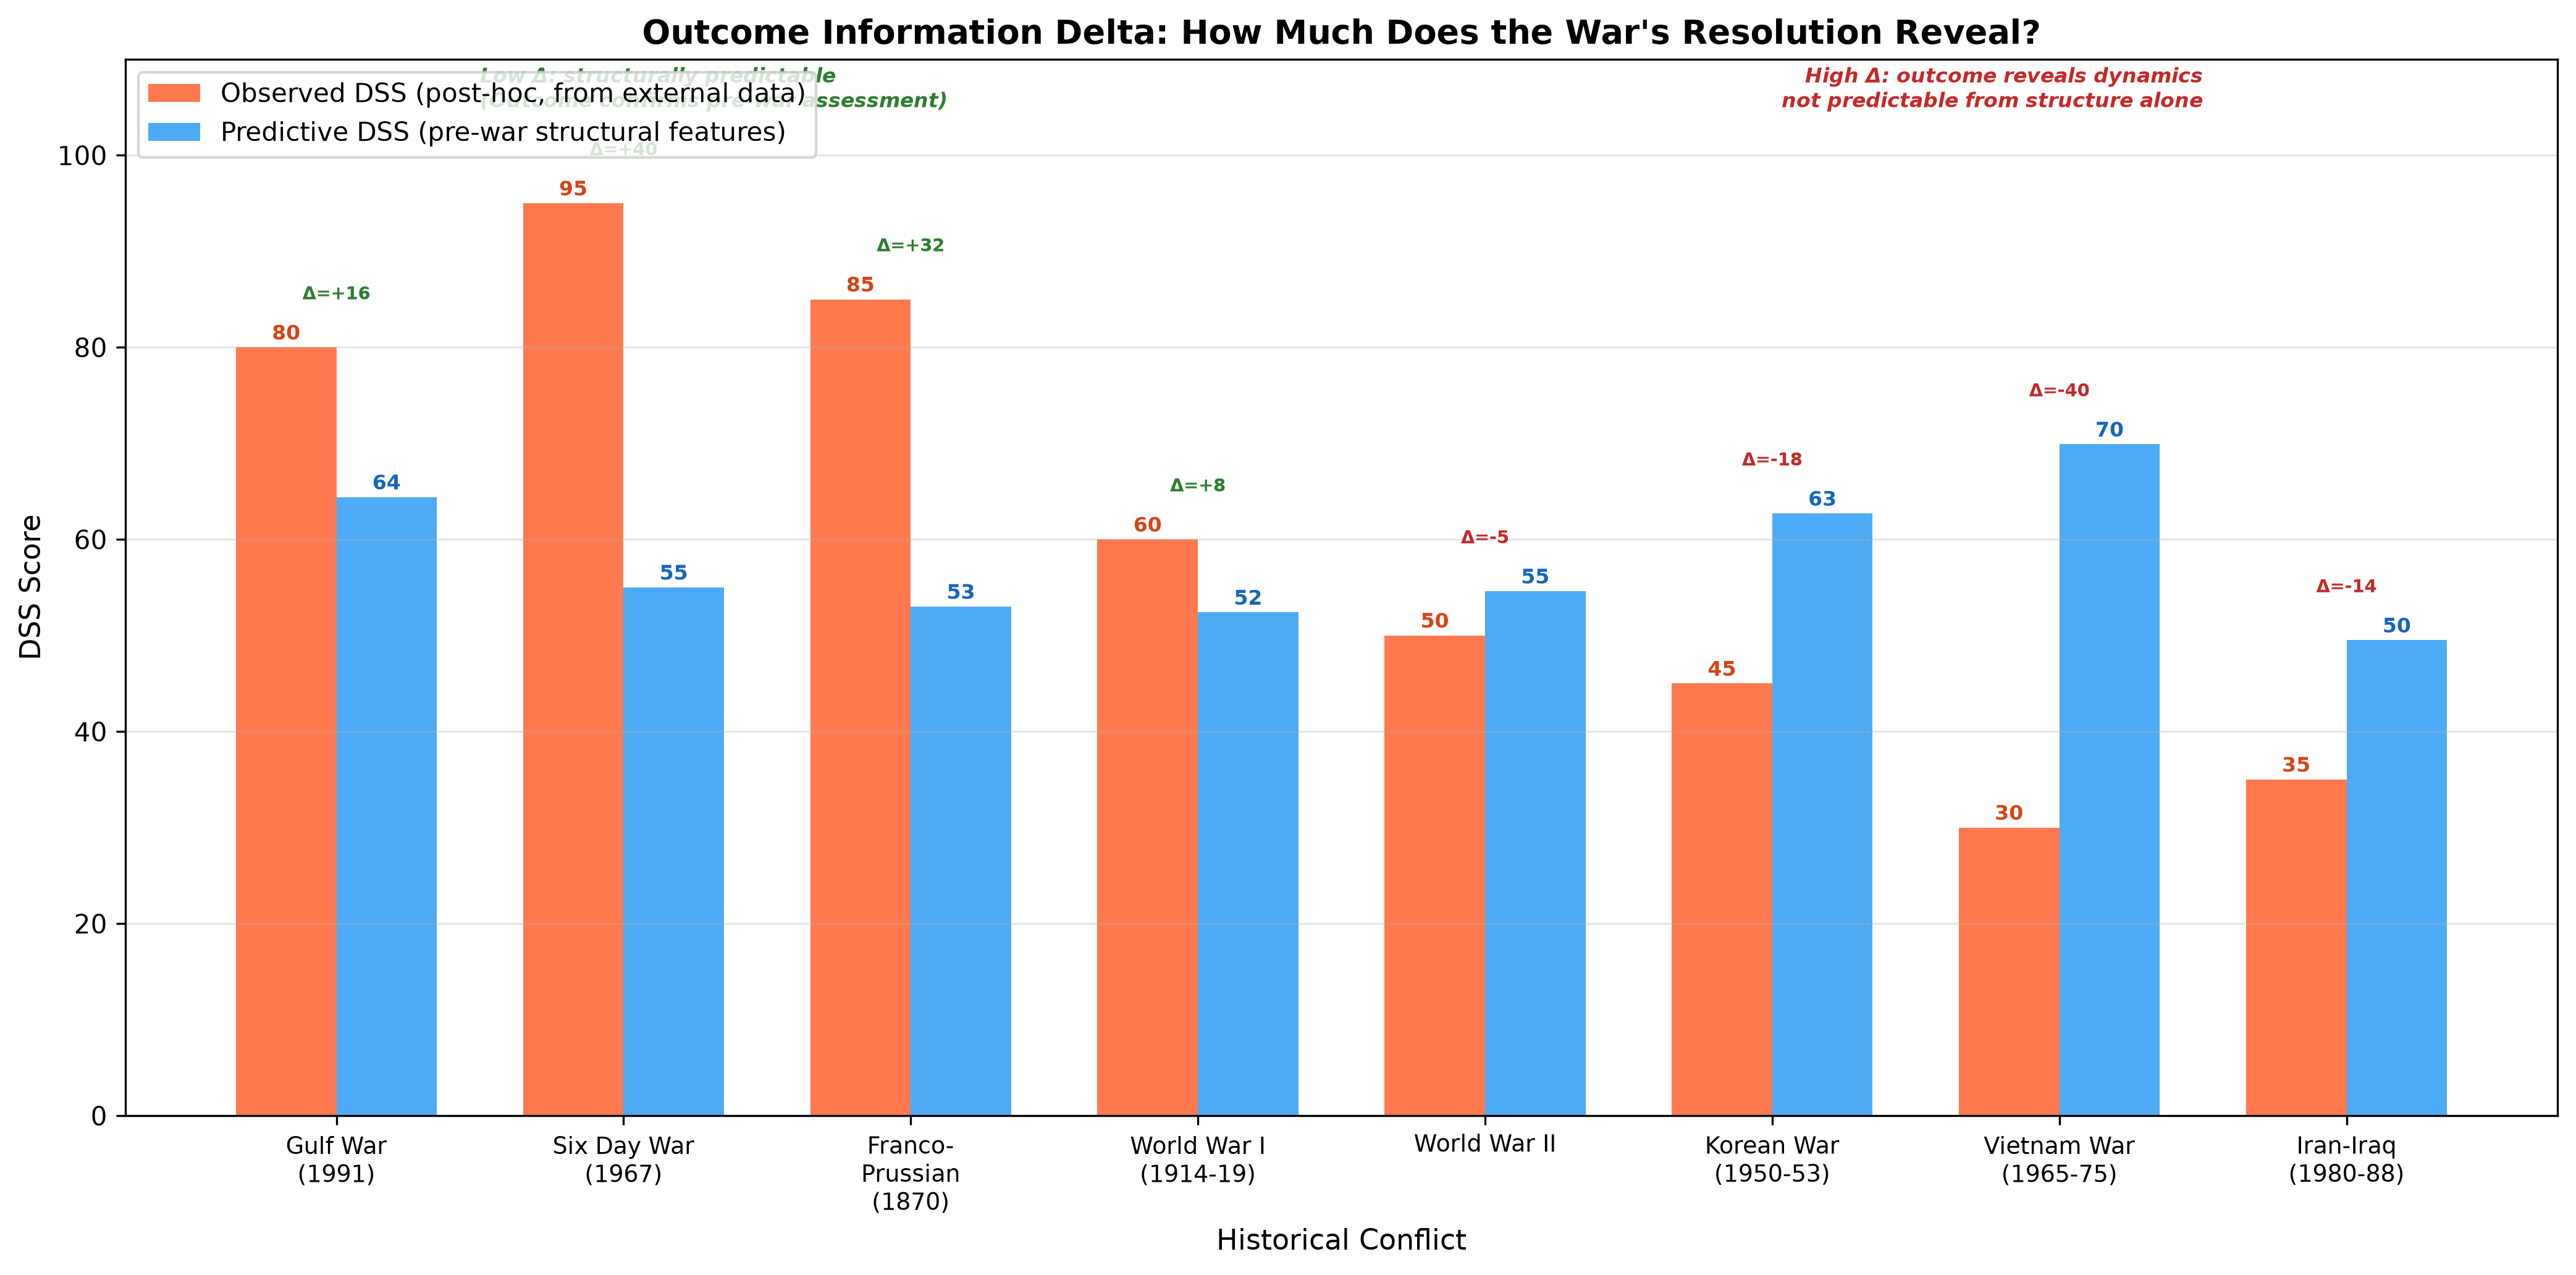
\includegraphics[width=0.8\textwidth]{figures/fig_02_observed_vs_predictive_dss.png}
\caption{Observed versus structural DSS proxy for eight historical cases. The observed-structural DSS gap measures how much additional information becomes available after conflict resolution. Negative gaps indicate that structural factors overpredict decisiveness relative to what actually occurred. The Six Day War shows the highest positive gap, indicating that the speed and totality of Israeli victory exceeded structural expectations.}
\label{fig:obs_pred_dss}
\end{figure}

The simulation-derived DSS (Equation~\ref{eq:sim_dss}) is a third variant that measures the simulation's own shock outputs. This metric is used only for internal model consistency checks and should not be interpreted as an empirical finding. We make this distinction explicit throughout the paper.

\subsubsection{Derived Metrics: DSS and SES from Simulation}

The simulation computes DSS and SES from the simulated state trajectory rather than from external data. DSS captures the magnitude of sudden military declines:

\begin{equation}
\text{DSS}_{\text{sim}}(t) = \min\!\Big(100,\;
  \frac{\max(0, -\Delta\text{Mil})}{\text{Mil}(0)} \cdot 50
  + \mathbb{1}[\text{Mil}(t) < 0.3 \cdot \text{Mil}(0)] \cdot 30
  + \mathbb{1}[\text{Pol}(t) < 20] \cdot 20\Big)
\label{eq:sim_dss}
\end{equation}

SES captures cumulative exhaustion across three dimensions plus duration:
\begin{equation}
\text{SES}_{\text{sim}}(t) = \Big(0.3 \cdot E_{\text{mil}}(t) + 0.3 \cdot E_{\text{econ}}(t) + 0.2 \cdot E_{\text{pol}}(t) + 0.2 \cdot \min(1, t/60)\Big) \cdot 100
\label{eq:sim_ses}
\end{equation}

\noindent where $E_{\text{mil}}(t) = 1 - \text{Mil}(t)/\text{Mil}(0)$, and analogously for economic and political exhaustion.

\subsubsection{Termination Conditions}

The simulation terminates when any of the following conditions is met: (1) political will drops below 10 for either side (political collapse); (2) military strength drops below 10 (military destruction); (3) one side holds a $2\!:\!1$ military advantage with the weaker side below 30 (dominance); (4) both sides reach $\text{SES} > 80$ (mutual exhaustion); (5) economic capacity drops below 15 for one side (economic collapse); or (6) both military values fall below 50 (negotiated settlement).

\subsection{Stochastic Noise Model}

The simulation adds independent Gaussian noise $\mathcal{N}(0, 0.5)$ to all state variables after each deterministic update step. This noise is \textbf{additive, not multiplicative}: it is applied after the deterministic attrition and shock updates, and state clamping to $[0, 100]$ occurs after noise addition. The noise term is not intended as an approximation to a stochastic differential equation; it represents small unmodeled shocks in a bounded discrete-time simulation. A Monte Carlo sensitivity analysis (500 seeds per historical preset) shows that four of seven cases are highly stable (dominant share $\geq$ 97\%), while three cases---World War I (62\%), World War II (77\%), and the Vietnam War (79\%)---show non-trivial noise sensitivity with two distinct termination outcomes across runs (see Appendix~\ref{app:noise_sensitivity}). The noise-sensitive cases should be interpreted as probabilistic rather than deterministic classifications.

\subsection{Termination Threshold Sensitivity}

The termination thresholds used in the hybrid classification rule (Equation~\ref{eq:hybrid}) and in the simulation termination conditions are heuristic decision rules in a bounded discrete-time model. They are not claims that historical collapse occurs at a universal numerical value. Table~\ref{tab:threshold_sensitivity_extra} reports sensitivity results for the simulation termination thresholds: political collapse threshold ($\{5, 10, 15\}$), military collapse threshold ($\{5, 10, 15\}$), dominance ratio ($\{1.5, 2.0, 2.5\}$), and settlement military threshold ($\{40, 50, 60\}$). The core mechanism classifications (Gulf War as decisive, Vietnam and WWI as exhaustion) are stable across all tested threshold combinations.

\begin{table}[H]
\centering
\caption{Simulation termination threshold sensitivity. Core case-study classifications remain stable across all tested threshold combinations.}
\label{tab:threshold_sensitivity_extra}
\small
\begin{tabularx}{\textwidth}{@{}l c c c X@{}}
\toprule
\textbf{Threshold} & \textbf{Values} & \textbf{Combos} & \textbf{Flips} & \textbf{Interpretation} \\
\midrule
Political collapse & 5, 10, 15 & 3 & 0 & All cases stable \\
Military collapse & 5, 10, 15 & 3 & 0 & All cases stable \\
Dominance ratio & 1.5, 2.0, 2.5 & 3 & 1 & Franco-Prussian sensitive at 2.5 \\
Settlement mil.\ threshold & 40, 50, 60 & 3 & 0 & Korean War stable \\
\bottomrule
\end{tabularx}
\end{table}

\subsection{Statistical Methods}

\subsubsection{Logistic Regression}

We use logistic regression as a deliberately simple baseline to test the predictive power of material-capability features for war duration category. The model takes the form:

\begin{equation}
\log\left(\frac{P(\text{Short})}{1 - P(\text{Short})}\right) = \beta_0 + \boldsymbol{\beta}^T \mathbf{X}
\end{equation}

\noindent where $\mathbf{X}$ is a vector of ten material-capability features: initial values and percentage changes for CINC scores, military expenditure, energy consumption, military personnel, and iron and steel production. Battle deaths are excluded because they are wartime outcomes, not ex-ante predictors. The target is binary: short war ($<$365 days) vs.\ long war ($\geq$365 days). We report 5-fold stratified cross-validation accuracy with standard deviation, balanced accuracy, precision, recall, F1 score, and AUC-ROC. The logistic regression serves as a linear baseline: its limited performance demonstrates that additive relationships among these features contain limited predictive information, while the random forest's improvement quantifies the information contained in nonlinear interactions.

\subsubsection{Random Forest Classification}

We train a random forest classifier (100 trees, max depth 5) on the same ten material-capability features to capture nonlinear interactions. Feature importance is measured by both Gini importance (mean decrease in impurity) and permutation importance (30 repeats on the held-out test set). We use 5-fold stratified cross-validation and report accuracy with standard deviation, balanced accuracy, AUC-ROC, and a full classification report. The random forest serves as the nonlinear structural model: its improvement over logistic regression quantifies the predictive information contained in feature interactions.

\subsubsection{Ablation Study}

To assess the independent contribution of DSS and SES, we conduct an ablation study comparing four model specifications:
\begin{enumerate}
    \item Baseline: controls only
    \item DSS-only: DSS + controls
    \item SES-only: SES + controls
    \item Full: DSS + SES + controls
\end{enumerate}

We compare models using likelihood ratio tests and report the change in AIC for each specification. The analysis reveals whether DSS and SES capture overlapping or distinct variance in termination type.

\subsubsection{Survival Analysis}

We apply Cox proportional hazards models to war duration data, testing whether DSS and SES scores predict the hazard of war termination. The analysis addresses the question of whether decisive shock dynamics are associated with shorter or longer wars.

\subsubsection{Threshold Sensitivity}

We conduct a systematic sensitivity analysis of the classification thresholds (minimum axis value, mixed threshold, and decisive/exhaustion margin) across 175 parameter combinations. For each combination, we compute the agreement rate with the current classification and measure category stability. This analysis determines whether the classification is robust to threshold choices or depends critically on specific values.

\subsection{Simulation Validity and Scope}

The dynamical simulation (Section~\ref{sec:simulation}) is a \textbf{bounded discrete-time iterative map}, not a system of differential equations fitted to empirical data. Its coefficients are literature-derived assumptions and heuristic normalization factors, not maximum-likelihood estimates. The simulation's validity is therefore limited to generating \emph{qualitatively consistent} conflict trajectories under specified parameter regimes: it can demonstrate that the interaction of shock and attrition mechanisms produces termination patterns consistent with historical records, but it cannot predict specific battle outcomes, dates of termination, or the precise sequence of events in any individual war.

The simulation is valid for:
\begin{itemize}
    \item Exploring how changes in shock frequency, attrition rate, and resilience parameters shift the balance between decisive and attritional regimes
    \item Demonstrating that DSS and SES can emerge from interacting processes rather than being imposed externally
    \item Generating synthetic trajectories that match aggregate qualitative features of historical wars (e.g., rapid collapse vs.\ prolonged stalemate)
\end{itemize}

The simulation is \textbf{not} valid for:
\begin{itemize}
    \item Forecasting specific battle outcomes or war termination dates
    \item Estimating causal effect sizes for real-world interventions
    \item Predicting which side will win a future conflict
    \item Serving as an empirical estimator of historical parameters
\end{itemize}

All simulation results should be interpreted at the \emph{regime} level: the qualitative distinction between decisive-shock-dominant and attritional-exhaustion-dominant parameter spaces, rather than the precise numerical values of DSS or SES scores for any individual case.

\subsection{Historical Reconstruction versus Blind Prediction}

We distinguish two evaluation strategies with fundamentally different epistemic status.

Historical mechanism classifications were assigned independently of individual simulation trajectories but were not blinded from the development team. They should therefore be interpreted as structured comparisons rather than independent validation labels.

\textbf{Calibrated reconstruction} tests whether mechanism combinations can generate trajectory classes consistent with historically observed patterns. For each historical preset, we set initial conditions and parameters to match observed pre-war conditions, then compare the simulated trajectory with historical records. This is equivalent to a historical case study or parameterized reconstruction; it demonstrates internal model consistency, not independent prediction. We explicitly do \emph{not} claim this constitutes validation in the predictive sense. As the model assumptions audit acknowledges, ``the preset encodes the hypothesis rather than testing it'' for some cases (e.g., the Franco-Prussian War preset has shock=90, attrition=35).

\textbf{Mechanism-trajectory classification} separates termination events from strategic causes. Instead of allowing the termination outcome string (e.g., ``decisive\_victory\_a'') to determine the mechanism label, the mechanism-trajectory classifier computes independent scores for decisive shock and strategic exhaustion based on the simulation trajectory. This classifier agrees with author-assigned labels in 6 of 7 cases (calibration consistency).

We report calibrated reconstruction and mechanism classification transparently, while treating independent blind prediction as future validation rather than as a result of the present paper.

We distinguish three categories of case usage: (1) \textbf{calibration cases}, whose parameters were tuned during model development; (2) \textbf{demonstration cases}, used to illustrate the framework but not tuned against; and (3) \textbf{holdout cases}, reserved for independent evaluation. The seven case studies in this paper include calibration cases (Gulf War, Franco-Prussian War) and demonstration cases (Vietnam, WWI, WWII, Korea, Iran--Iraq). No independent holdout validation of the mechanism labels is claimed in this version. A future validation protocol should use a pre-registered holdout split unavailable to model calibration (see Section~\ref{sec:validation_protocol}).

\subsection{Proposed Independent Validation Protocol}\label{sec:validation_protocol}

The falsification criteria in Section~\ref{sec:falsification_section} identify independent blind validation as the most important future test. We describe a concrete protocol here to enable replication.

\textbf{Step 1: Holdout selection.} Select a stratified random sample of 50+ wars from the IWB dataset with complete battle-level data. Stratify by era (pre-1900, 1900--1945, post-1945) and termination type (decisive, exhaustion, negotiated). Reserve these cases entirely from model development; do not use them for calibration, threshold tuning, or demonstration.

\textbf{Step 2: Blinded mechanism labeling.} Three or more independent historians, blind to model outputs, assign each holdout case a mechanism label (decisive shock, strategic exhaustion, mixed/uncertain) using a structured coding protocol. The protocol should specify: (a) the definition of ``dominant mechanism'' as the factor that made the losing side's position unwinnable; (b) a checklist of observable indicators for each mechanism class; and (c) inter-rater reliability targets (Fleiss' kappa $\geq 0.40$).

\textbf{Step 3: Model classification.} Apply the DSS/SES hybrid classifier (Equation~\ref{eq:hybrid}) to the holdout cases using only pre-outcome information for the structural DSS proxy components. Report exact-match accuracy and Cohen's kappa between historian labels and classifier labels.

\textbf{Step 4: Evaluation.} The framework is falsified if exact-match accuracy falls below 20\% (criterion 2) or Fleiss' kappa falls below 0.40 (criterion 5). Partial success (50--79\% accuracy) would indicate the framework captures signal but requires refinement. Success ($\geq$80\% accuracy with kappa $\geq$0.60) would constitute strong independent evidence for the attritional iceberg thesis.

This protocol is pre-specified but not yet executed. Results from this validation will be reported in a subsequent publication.
